\subsection{Transverse isotropic elastic tensile test}
\label{subsec:Me7}

\subsubsection{Definition}
\label{subsubsec:Me7_def}

Tension of a quadratic plate according to Schr\"oder \cite{Schroeder:1996}, Kohlmeier \cite{Kohlmeier:2006} and Fiolka \cite{Fiolka:2007} is carried out to verify the linear elastic transverse isotropic material model. Within this context, a laminated material structure perpendicular to the plane under consideration is assumed. The direction of anisotropy within this plane, which is defined by a vector $\miu{a}{}{}$ is perpendicularly oriented to the material layers.

\subsubsection{Solution}
\label{subsubsec:Me7_sol}

During simulation, the direction of anisotropy is rotated counterclockwise starting with an angle $\varphi$ of $\varphi=0^{\circ}$ and ending with $\varphi=180^{\circ}$. Consequently, as in OpenGeoSys the direction of anisotropy is assumed to be directed parallel to the local $\bar{y}$-axis, and the angle of rotation is defined as the rotation between the global $x$-axis and the local $\bar{x}$-axis, the input angle changes in the range of $\varphi=-90^{\circ}$\dots$90^{\circ}$.

Assuming plane strain conditions for the twodimensional case, the quadratic plate has an edge length of $l=10\,$mm, and was analyzed using triangular and rectangular elements respectively. For details of this model (geometry, boundary conditions, material orientation) see Fig.~\ref{Me_tens_transiso_model_2d}.

\begin{figure}[!htb]
\begin{center}
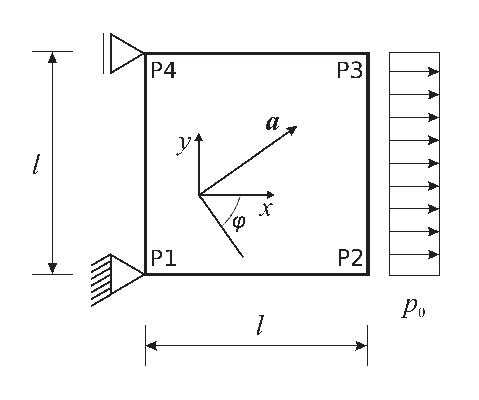
\includegraphics[scale=0.95]{PART_II/M/tenstest_model_mod.eps}
\end{center}
\caption{Tensile test. Model definition according to Kohlmeier \cite{Kohlmeier:2006}. Vector $\miu{a}{}{}$ defines the direction of anisotropy.}
\label{Me_tens_transiso_model_2d}
\end{figure}

To verify the linear elastic transverse isotropic material model in the threedimensional case, the tensile test was simulated using a rectangular sample with an edge length $l=10\,$mm and a height $h=1\,$mm. According to the twodimensional case, a vertically arranged laminated material structure is assumed. The direction of anisotropy, which is defined by a vector $\miu{a}{}{}$ is perpendicularly oriented to the material layers. During simulation, the direction of anisotropy is rotated counterclockwise in the $xy$-plane from $\varphi=0^{\circ}$ to $\varphi=180^{\circ}$. 

Within the context of the different opportunities offered by the input structure of OpenGeoSys to define the anisotropy direction, the coefficients of the unit normal vector which is parallel to the direction of anisotropy are given as $n_x=\cos\varphi$, $n_y=\sin\varphi$, and $n_z=0$. Considering the case that the basis vectors of the local Cartesian coordinate system for transverse isotropic materials are provided by consecutive rotations of the plane of isotropy about the global $y$($x_2$)-axis and the $\bar{x}$($\bar{x}_1$)-axis of the once rotated system, the angle $\alpha$ has a constant value of $90^{\circ}$, whereas the angle $\beta$ changes from $0^{\circ}$ to $-180^{\circ}$. Using the angles known from applications in structural geology to generate the constitutive rotation matrices, the dip $\phi$ has the constant value of $90^{\circ}$, and the azimuth varies from $90^{\circ}$\dots$0^{\circ}$ (for $0^{\circ}\leq\varphi\leq 90^{\circ}$) and $360^{\circ}$\dots$270^{\circ}$ (for $90^{\circ}\leq\varphi\leq 180^{\circ}$) respectively. For details of the threedimensional model (geometry, boundary conditions, material orientation) see Fig.~\ref{Me_tens_transiso_model_3d}.

\begin{figure}[!htb]
\begin{center}
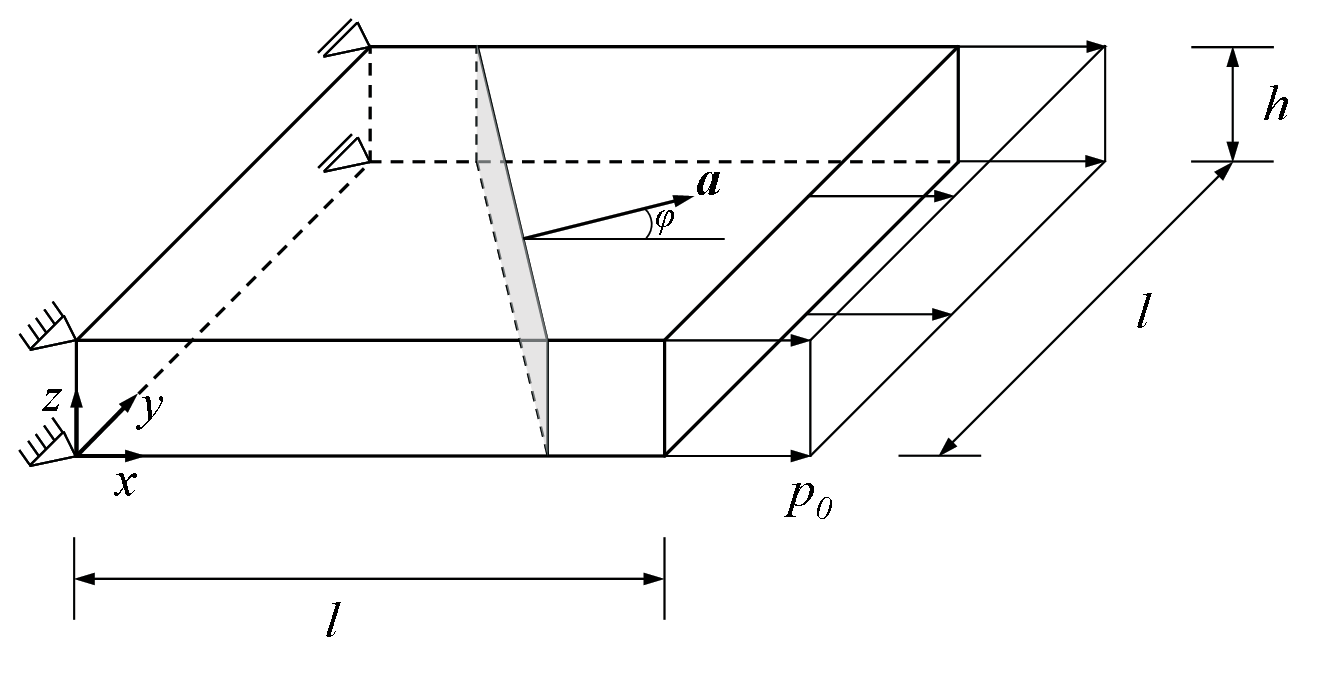
\includegraphics[width=0.85\textwidth]{PART_II/M/tenstest_model_3D.eps}
\end{center}
\caption{Tensile test. Threedimensional model definition according to Fiolka \cite{Fiolka:2007}. Vector $\miu{a}{}{}$ defines the direction of anisotropy.} 
\label{Me_tens_transiso_model_3d}
\end{figure}

Initial conditions do not have to be given for the problem under consideration. The left-hand edge is fixed in horizontal direction. To avoid rigid body motions, the left lower corner node is fixed in both vertical and horizontal directions. A distributed tension load of $p_0=0.2\,$Mpa is applied at the right-hand edge. In the threedimensional case, the plane strain condition was realized preventing any displacement in $z$-direction on the upper and lower boundary surfaces of the sample.

The material parameters are summarized in Tab.~\ref{Me_matpar_transiso_tens}.

\begin{table}[!htb]
\centering
\caption{Material parameters}
\label{Me_matpar_transiso_tens}
\begin{tabular}{llll}
\toprule
Symbol & Parameter & Value & Unit \\
\midrule
$E_i$      & Young's modulus & $\ \,561.12$ & MPa \\
$E_a$      & Young's modulus & $1311.83$    & MPa \\
$\nu_i$    & Poisson's ratio & $\ \,0.6032$ & --  \\
$\nu_{ia}$ & Poisson's ratio & $\ \,0.1838$ & --  \\
$G_a$      & Shear modulus   & $\ \,375.00$ & MPa \\
\bottomrule
\end{tabular}
\end{table}

\clearpage

\subsubsection{Results}
\label{subsubsec:Me7_res}

The numerical results obtained with {\sl OpenGeoSys} are compared to values given in \cite{Kohlmeier:2006}. They include displacement coefficients of various corner nodes of the plate depending on the anisotropy direction, and show a good agreement (cf. Fig.~\ref{Me_tens_transiso_test_2d}). 
%
\begin{figure}[!htb]
\begin{center}
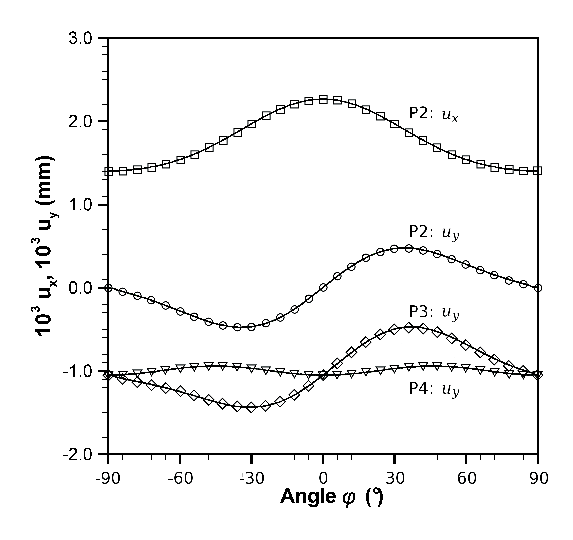
\includegraphics[scale=0.7]{PART_II/M/tenstest_results_OGS.eps}
\end{center}
\caption{Tensile test. {\sl OpenGeoSys} results (symbols) at length $l=10\,$mm and an edge load of $p_0=0.2\,$Mpa compared to the reference solution given by Schr\"oder \cite{Schroeder:1996} and Kohlmeier \cite{Kohlmeier:2006} (continuous lines).}
\label{Me_tens_transiso_test_2d}
\end{figure}

\clearpage